\section{Real-to-Sim-to-Real Pipeline}
\label{sec:method}

\begin{figure*}[t]
    \centering
    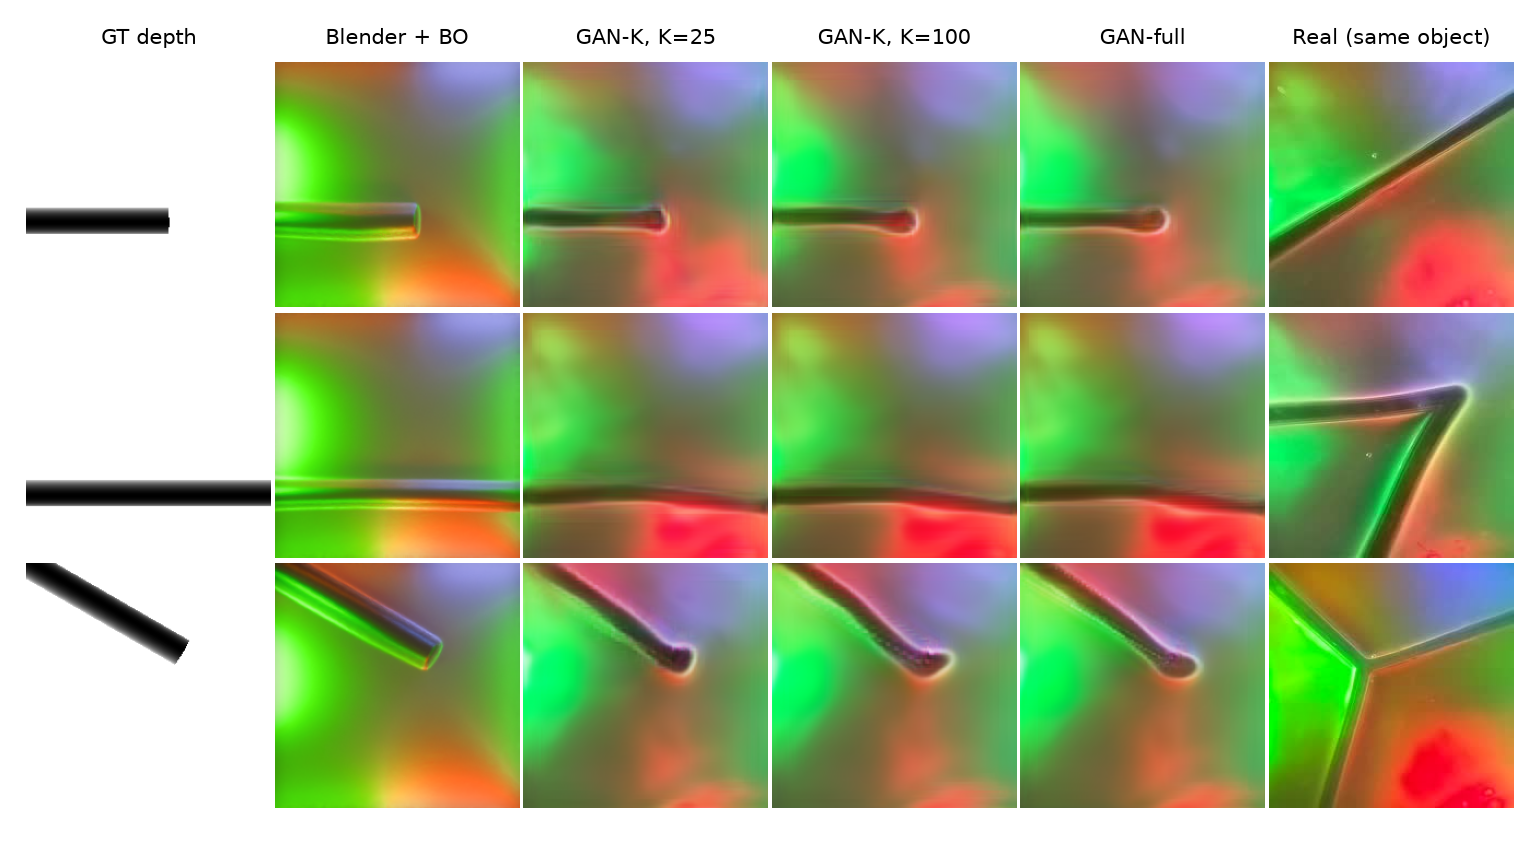
\includegraphics[width=0.96\textwidth]{figures/fig_renders.png}
    \caption{\textbf{Two renderers, one contact.} Each row is one simulated contact (GT depth, left) rendered by the physically calibrated Blender renderer, by the learned renderer trained on $\Kreal=25$ or $\Kreal=100$ real pairs per object, and by the learned renderer trained on all real pairs (GAN-full). The right column shows a real frame of the same object. The physical renderer reproduces the illumination field but not the dark, low-contrast contact shading of the real gel; the learned renderers reproduce the shading and inherit the mean illumination field of their training frames.}
    \label{fig:renders}
\end{figure*}

\subsection{Problem Statement}
Let $M$ be an object mesh and $q$ a contact state (planar pose of the object relative to the sensor and indentation depth). A tactile renderer $\mathcal{R}_\theta$ maps $(M,q)$ to an image and dense labels,
\begin{equation}
    (\hat I, D, N) = \mathcal{R}_\theta(M,q),
\end{equation}
where $D$ is the contact depth map, $N$ the surface normal map and $\theta$ the appearance parameters. The geometry part $\mathcal{G}:(M,q)\mapsto(D,N)$ is shared by every renderer we study; renderers differ only in the appearance operator $\mathcal{P}_\theta:(D,N)\mapsto\hat I$ and in the real data $\mathcal{D}^{r}_{\mathrm{cal}}$ used to fit $\theta$. A downstream model $f_\phi$ predicts $(\hat D,\hat N,\hat p)$ from a real image, with $p$ the planar pose. We measure the utility of a renderer by the real test error of $f_\phi$ after training on synthetic data $\mathcal{D}_{\mathrm{sim}}^{\theta}$ together with a real subset $\mathcal{D}^{r}_{\mathrm{task}}$, and we control the total real budget $\mathcal{D}^{r}_{\mathrm{cal}}\cup\mathcal{D}^{r}_{\mathrm{task}}$.

\subsection{Sensor and Data}
\noindent\textbf{Sensor.} We use \sensor{}, a GelSlim-type fingertip sensor with a $17.5\,$mm square gel view imaged by an internal camera under six colored LED emitters. Images are center-cropped to $0.816$ of the view and resized to $224\times224$.

\noindent\textbf{Real data.} A KUKA LBR Med arm presses the sensor onto 12 ridge-pattern objects (line, cross and rod patterns of known geometry), recording the tactile image and end-effector pose at every contact. A reference-object calibration relates object pose to the sensor frame; depth and normal references are computed from the mesh at the recorded pose, so they are geometric targets rather than membrane measurements. After filtering frames whose image-derived contact region disagrees with the reference (IoU $<0.3$), $4{,}669$ frames remain ($222$--$568$ per object). Each object was captured in one session, so \emph{object identity and capture session coincide}; we return to this in Sec.~\ref{sec:negative}. Every tenth frame is held out as the real validation split ($472$ frames).

\noindent\textbf{Contact sampler.} For each object we sample contact cells over the mesh at 12 base rotations ($30^\circ$ apart), an indentation depth of $0.8$--$1.2\,$mm and a small in-plane jitter, and export the depth map $D$ from the object z-buffer and $N$ by finite differences. Simulated poses are restricted to each object's real rotation and translation ranges (margin $1.5\times$). The same $5{,}345$ simulated contacts feed every renderer.

\subsection{Physically Calibrated Renderer}
\label{sec:blender}
The physical renderer is implemented in Blender/Cycles. Gel deformation is geometric: a gel surface mesh is shrink-wrapped onto the object along the sensor normal and smoothed with 35 corrective-smoothing iterations to mimic elastomer stiffness. The gel material is a glossy/transparent mix (roughness $0.45$, glossy fraction $0.17$) with a contact-darkening term driven by gel height. Illumination comes from six area emitters with individual strength and RGB color. A post-processing stage adds saturation, brightness, contrast, haze and a low-frequency gel-warp field.

\noindent\textbf{Calibration from one frame.} Following the base-field alignment of inverse tactile rendering, we fit $\theta_{\mathrm{illum}}\cup\theta_{\mathrm{post}}$ (three emitters $\times$ (strength, R, G, B) plus four post-processing scalars; 16 parameters) by minimizing
\begin{equation}
    \mathcal{L}_{\mathrm{base}} = 0.6\,\|B^{r}-\hat B_\theta\|_2^2 + 0.4\,D_{\mathrm{Bhat}}\!\left(H(B^{r}),H(\hat B_\theta)\right)
\end{equation}
between the real no-contact image $B^{r}$ and the rendered one, with $H$ the per-channel histogram and $D_{\mathrm{Bhat}}$ the Bhattacharyya distance, using tree-based Bayesian optimization (500 evaluations, warm-started from manual tuning). The remaining gel and contact parameters were tuned by hand on a few contact frames. The real budget of this renderer is therefore \emph{one no-contact frame}, and it never sees a labeled contact.

\subsection{Learned Renderer}
\label{sec:gan}
The learned renderer replaces $\mathcal{P}_\theta$ by a conditional GAN~\cite{isola2017pix2pix,church2022tactile}. The generator is a five-level U-Net taking the depth map and two CoordConv coordinate channels (the illumination field is a function of position) and producing an RGB image; the discriminator is a $70\times70$ PatchGAN with spectral normalization on the (depth, image) pair. The loss is adversarial + $100\,(\mathrm{L1} + \mathrm{gradient\;L1} + \mathrm{low\text{-}frequency\;L1})$. At data-generation time the simulated depth is jittered by $\pm15\%$ before rendering.

\noindent\textbf{Real budget.} We train one generator per budget: GAN-$\Kreal$ uses $\Kreal$ real (depth, image) pairs per object, drawn as an evenly spaced subset of each object's training frames; GAN-LOO uses all training frames of the 9 non-held-out objects; GAN-full uses all $4{,}197$ training pairs. Small budgets are trained for at least $30$k generator updates. The GAN-$\Kreal$ subset is by construction \emph{the same} $\Kreal$ frames the downstream model later receives (Sec.~\ref{sec:protocol}).

\subsection{Downstream Tactile Model}
The downstream model is deliberately simple and identical for every renderer: a frozen sensor-invariant tactile encoder (SITR-B/18~\cite{gupta2025sitr}, ViT-B/16, 18 calibration images) provides patch tokens at four depths; a DPT decoder~\cite{ranftl2021dpt} predicts depth and normals at $224\times224$; a pose head pools the class token with the mean patch token and regresses $(\cos\theta,\sin\theta,t_x,t_y)$. Only the decoder, pose head and a learned object embedding are trained ($12$M parameters). Losses are MSE on depth and normals, $1-\cos(\theta-\hat\theta)$ on rotation and L1 on translation, balanced by grouped uncertainty weighting~\cite{kendall2018multi}. Training co-mixes simulated and real frames in one dataset; simulated frames receive photometric augmentation (gain, bias, gradient, noise) and $\pm15^\circ$ gel-spin rotation with matched label rotation, real frames receive none. AdamW, learning rate $2\times10^{-4}$, batch 32, cosine schedule with 1k warm-up steps. \todo{Pilot tables use 50 epochs; final tables will use 150 epochs (runs in progress). A 150-epoch check on four key configurations changed no conclusion.}

\subsection{Leakage-Controlled Protocol}
\label{sec:protocol}
Two protocols, one rule: \emph{no frame used to evaluate $f_\phi$ is ever seen by the renderer.}

\noindent\textbf{Leave-object-out (LOO).} Three objects (a two-line, a rod and a cross pattern; $1{,}244$ frames) are removed from all real training. They are never used to calibrate a renderer, never appear as real frames in downstream training, and are evaluated in full. Checkpoints are selected on the validation split of the nine remaining objects. Simulated contacts of the three meshes are available to every renderer, mimicking the deployment case ``new object with a CAD model but no real touches''. A \emph{geometry control} additionally removes the three meshes from simulation.

\noindent\textbf{$\Kreal$-shot.} Every object contributes $\Kreal\in\{0,10,25,100\}$ evenly spaced real training frames. The learned renderer is trained on exactly those frames; the downstream model co-trains on those frames plus simulated data (or on those frames alone, with the same number of updates). Evaluation is on the standard real validation split.

\noindent\textbf{Leaky reference.} To quantify the bias of the common practice, we also report GAN-full (renderer trained on all real pairs) in both protocols. In LOO its training set contains the held-out objects; in $\Kreal$-shot it contains frames adjacent to the validation frames. We mark these rows as leaky and never bold them.

\noindent\textbf{Metrics.} Depth MSE over all pixels ($\mathrm{mm}^2$), the metric used by prior work on this sensor; and, because $\approx90\%$ of pixels are non-contact background, the mean absolute error inside the reference contact region (contact MAE, mm), contact IoU (predicted depth $>0.05\,$mm vs.\ reference $>0$), and the per-frame peak-depth error. For pose: mean angular error and normalized translation L1.
